\documentclass[12pt]{article}
\usepackage{amsfonts, amssymb, amsmath, amsthm}
\usepackage[margin=1in]{geometry}
\usepackage{tikz}
\usetikzlibrary{patterns, decorations.pathreplacing, arrows.meta, calc}

\pagestyle{myheadings}
\markright{Explainer: Rudin 1.18 — Orthogonal Vectors in $\mathbb{R}^k$\hfill}

\newcommand{\R}{\mathbb{R}}
\newcommand{\vx}{\mathbf{x}}
\newcommand{\vy}{\mathbf{y}}

\begin{document}

\begin{center}
    \textbf{\Large Orthogonal Vectors in $\mathbb{R}^k$}\\[0.5em]
    \large A visual guide to Rudin 1.18
\end{center}

\section{The Claim}

If $k \geq 2$ and $\vx \in \mathbb{R}^k$, there exists $\vy \neq \mathbf{0}$ such that $\vx \cdot \vy = 0$.

This says: in 2 or more dimensions, every vector has a nonzero \textbf{perpendicular} vector.

\section{What Does $\vx \cdot \vy = 0$ Mean?}

The dot product $\vx \cdot \vy = x_1 y_1 + x_2 y_2 + \cdots + x_k y_k$.

When $\vx \cdot \vy = 0$, we say $\vx$ and $\vy$ are \textbf{orthogonal} (perpendicular).

\begin{center}
\begin{tikzpicture}[scale=1.2]
    % Axes
    \draw[thick, ->] (-0.5, 0) -- (4, 0) node[right] {$x_1$};
    \draw[thick, ->] (0, -0.5) -- (0, 3) node[above] {$x_2$};

    % Vector x
    \draw[thick, blue, ->, >=stealth] (0, 0) -- (3, 1);
    \node[blue] at (3.2, 1.2) {$\vx$};

    % Vector y (perpendicular)
    \draw[thick, red, ->, >=stealth] (0, 0) -- (-0.5, 1.5);
    \node[red] at (-0.7, 1.7) {$\vy$};

    % Right angle symbol
    \draw (0.3, 0.1) -- (0.2, 0.4) -- (-0.1, 0.3);

    \node at (1.5, -1) {$\vx \cdot \vy = 0$ means $\vx \perp \vy$};
\end{tikzpicture}
\end{center}

\section{The Construction in $\mathbb{R}^2$}

Given $\vx = (x_1, x_2)$, we want $\vy = (y_1, y_2)$ with $\vy \neq \mathbf{0}$ and $x_1 y_1 + x_2 y_2 = 0$.

\textbf{Case 1:} If $x_2 \neq 0$, let $\vy = (1, -x_1/x_2)$

Check: $\vx \cdot \vy = x_1 \cdot 1 + x_2 \cdot (-x_1/x_2) = x_1 - x_1 = 0$ \checkmark

\textbf{Case 2:} If $x_2 = 0$, let $\vy = (0, 1)$

Check: $\vx \cdot \vy = x_1 \cdot 0 + 0 \cdot 1 = 0$ \checkmark

\begin{center}
\begin{tikzpicture}[scale=1]
    % Case 1
    \begin{scope}[xshift=-4cm]
        \draw[thick, ->] (-1, 0) -- (3, 0);
        \draw[thick, ->] (0, -1) -- (0, 2.5);

        \draw[thick, blue, ->, >=stealth] (0, 0) -- (2, 1);
        \node[blue] at (2.2, 1.2) {$\vx = (2, 1)$};

        \draw[thick, red, ->, >=stealth] (0, 0) -- (1, -2);
        \node[red] at (1.5, -1.8) {$\vy = (1, -2)$};

        \node at (1, -3) {\small Case 1: $x_2 \neq 0$};
    \end{scope}

    % Case 2
    \begin{scope}[xshift=4cm]
        \draw[thick, ->] (-1, 0) -- (3, 0);
        \draw[thick, ->] (0, -1) -- (0, 2.5);

        \draw[thick, blue, ->, >=stealth] (0, 0) -- (2, 0);
        \node[blue] at (2.3, 0.3) {$\vx = (2, 0)$};

        \draw[thick, red, ->, >=stealth] (0, 0) -- (0, 1.5);
        \node[red] at (0.4, 1.7) {$\vy = (0, 1)$};

        \node at (1, -3) {\small Case 2: $x_2 = 0$};
    \end{scope}
\end{tikzpicture}
\end{center}

\section{Extending to $\mathbb{R}^k$ ($k \geq 2$)}

The same idea works! We only use the first two coordinates.

Given $\vx = (x_1, x_2, x_3, \ldots, x_k)$:

\textbf{Case 1:} If $x_2 \neq 0$, let $\vy = (1, -x_1/x_2, 0, 0, \ldots, 0)$

\textbf{Case 2:} If $x_2 = 0$, let $\vy = (0, 1, 0, 0, \ldots, 0)$

In both cases, $\vx \cdot \vy = 0$ and $\vy \neq \mathbf{0}$.

\section{Why Does $k \geq 2$ Matter?}

In $\mathbb{R}^1$, vectors are just numbers. If $x \neq 0$:
\[
xy = 0 \quad \Rightarrow \quad y = 0
\]

\begin{center}
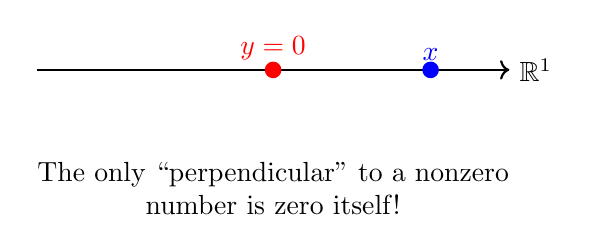
\begin{tikzpicture}[scale=1]
    \draw[thick, ->] (-3, 0) -- (3, 0) node[right] {$\mathbb{R}^1$};

    \fill[blue] (2, 0) circle (3pt) node[above] {$x$};
    \fill[red] (0, 0) circle (3pt) node[above] {$y = 0$};

    \node[text width=6cm, align=center] at (0, -1.5) {The only ``perpendicular'' to a nonzero\\number is zero itself!};
\end{tikzpicture}
\end{center}

In higher dimensions, there's ``room'' to be perpendicular.

\section{Geometric Intuition}

\begin{center}
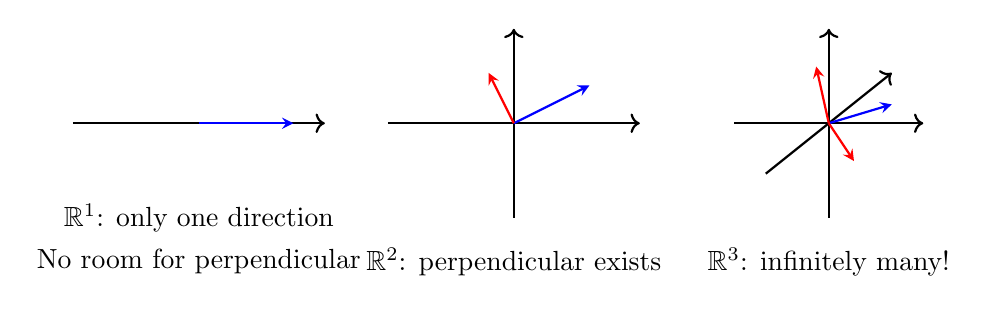
\begin{tikzpicture}[scale=0.8]
    % R^1
    \begin{scope}[xshift=-5cm]
        \draw[thick, ->] (-2, 0) -- (2, 0);
        \draw[thick, blue, ->, >=stealth] (0, 0) -- (1.5, 0);
        \node at (0, -1.5) {$\mathbb{R}^1$: only one direction};
        \node at (0, -2.2) {No room for perpendicular};
    \end{scope}

    % R^2
    \begin{scope}[xshift=0cm]
        \draw[thick, ->] (-2, 0) -- (2, 0);
        \draw[thick, ->] (0, -1.5) -- (0, 1.5);
        \draw[thick, blue, ->, >=stealth] (0, 0) -- (1.2, 0.6);
        \draw[thick, red, ->, >=stealth] (0, 0) -- (-0.4, 0.8);
        \node at (0, -2.2) {$\mathbb{R}^2$: perpendicular exists};
    \end{scope}

    % R^3
    \begin{scope}[xshift=5cm]
        \draw[thick, ->] (-1.5, 0) -- (1.5, 0);
        \draw[thick, ->] (0, -1.5) -- (0, 1.5);
        \draw[thick, ->] (-1, -0.8) -- (1, 0.8);
        \draw[thick, blue, ->, >=stealth] (0, 0) -- (1, 0.3);
        \draw[thick, red, ->, >=stealth] (0, 0) -- (-0.2, 0.9);
        \draw[thick, red, ->, >=stealth] (0, 0) -- (0.4, -0.6);
        \node at (0, -2.2) {$\mathbb{R}^3$: infinitely many!};
    \end{scope}
\end{tikzpicture}
\end{center}

In $\mathbb{R}^k$ with $k \geq 2$, the set of vectors perpendicular to $\vx$ forms a $(k-1)$-dimensional subspace — plenty of nonzero options!

\section{Summary}

\begin{center}
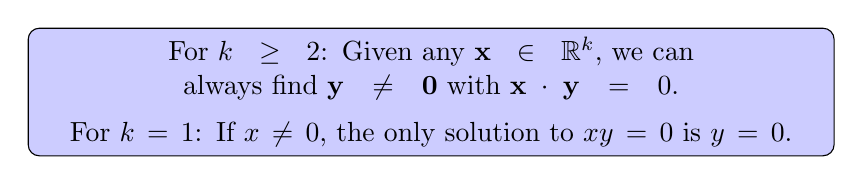
\begin{tikzpicture}
    \node[draw, rounded corners, fill=blue!20, text width=10cm, align=center] at (0, 0) {
        For $k \geq 2$: Given any $\vx \in \mathbb{R}^k$, we can always find $\vy \neq \mathbf{0}$ with $\vx \cdot \vy = 0$.\\[0.5em]
        For $k = 1$: If $x \neq 0$, the only solution to $xy = 0$ is $y = 0$.
    };
\end{tikzpicture}
\end{center}

\end{document}
